
\documentclass[tikz, border=10pt]{standalone}
\usepackage{tikz}
\usetikzlibrary{positioning, chains, shapes.geometric, fit, shapes, arrows.meta, calc, backgrounds}

\begin{document}
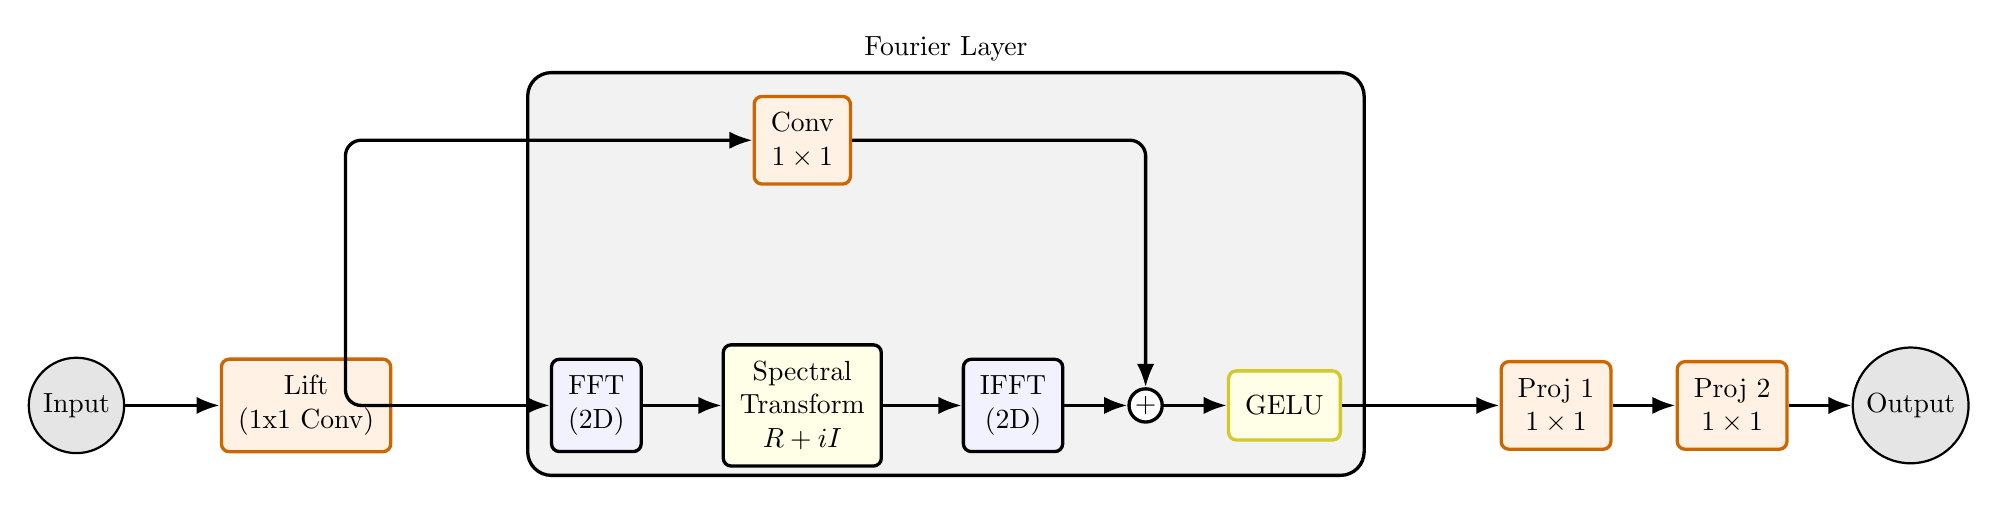
\begin{tikzpicture}[
    >=LaTeX, 
    very thick,
    node distance=1.0cm and 1.2cm,
    arrow/.style={
        ->,
        very thick,
        rounded corners=0.2cm
    },
    block/.style={
        rectangle,
        fill=gray!10,
        rounded corners=3mm,
        draw,
        very thick,
        inner sep=0.8em
    },
    layer/.style={
        rectangle,
        fill=white!10,
        rounded corners=1mm,
        inner xsep=0.6em,
        inner ysep=0.6em,
        minimum height=3.0em,
        align=center,
        draw,
        very thick
    },
    conv/.style={
        layer,
        fill=orange!10,
        draw=orange!80!black
    },
    relu/.style={
        layer,
        fill=yellow!10,
        draw=yellow!80!black,
        minimum height=2.5em
    },
    pool/.style={
        layer,
        fill=red!10,
        draw=red!80!black
    },
    input/.style={ 
        circle,
        minimum width=3.0em,
        draw,
        fill=gray!20,
        thick,
        align=center
    },
    sum/.style={
        circle,
        draw,
        fill=white,
        inner sep=0pt,
        minimum size=1.2em,
        node contents={+}
    }
]


    \node[input] (in) {Input};
    
    % Lift
    \node[conv, right=of in] (lift) {Lift\\(1x1 Conv)};
    \draw[arrow] (in) -- (lift);

    % Fourier Layer Detail
    \node[layer, right=2.0cm of lift, fill=blue!5] (fft) {FFT\\(2D)};
    \node[layer, right=1.0cm of fft, fill=yellow!10] (weights) {Spectral\\Transform\\$R + iI$};
    \node[layer, right=1.0cm of weights, fill=blue!5] (ifft) {IFFT\\(2D)};
    
    % Skip (W)
    \node[conv, above=2.0cm of weights] (w_skip) {Conv\\$1\times 1$};
    
    % Sum
    \node (sum) [sum, right=0.8cm of ifft];
    \node[relu, right=0.8cm of sum] (act) {GELU};

    \begin{scope}[on background layer]
        \node[block, fit=(fft) (ifft) (w_skip) (act), label=above:Fourier Layer] (fno_layer) {};
    \end{scope}

    % Connections
    \draw[arrow] (lift) -- (fft);
    \draw[arrow] (fft) -- (weights);
    \draw[arrow] (weights) -- (ifft);
    \draw[arrow] (ifft) -- (sum);
    \draw[arrow] (sum) -- (act);
    
    % Skip path
    \draw[arrow] (lift) -- ++(0.5,0) |- (w_skip.west);
    \draw[arrow] (w_skip.east) -| (sum.north);

    % Projection
    \node[conv, right=2.0cm of act] (proj1) {Proj 1\\$1\times 1$};
    \node[conv, right=0.8cm of proj1] (proj2) {Proj 2\\$1\times 1$};
    \node[input, right=0.8cm of proj2] (out) {Output};

    \draw[arrow] (act) -- (proj1);
    \draw[arrow] (proj1) -- (proj2);
    \draw[arrow] (proj2) -- (out);

\end{tikzpicture}
\end{document}
